\documentclass[tikz]{standalone}
\input{../tikz.tex.preamble}
\input{../colours.tex.preamble}

\begin{document}
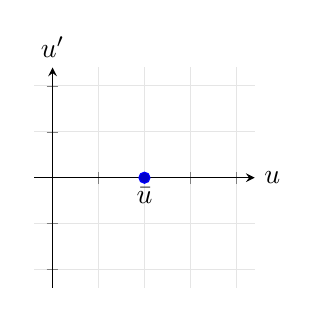
\begin{tikzpicture}
  \begin{axis}[
  axis lines = middle, % boxed, middle
  axis equal image,
  width={2in},
  %
  % domain and range
  %
  xmin={0}, xmax={4},
  ymin={-2}, ymax={2},
  enlargelimits=true,
  %
  % axis labels
  %
  xlabel={\(u\)}, xlabel style={anchor=west},
  ylabel={\(u'\)}, ylabel style={anchor=south},
  label style={at={(ticklabel* cs:1)}},
  %
  % ticks
  %
  xtick={0,1,...,4}, xticklabels={\empty},
  ytick={-2,-1,...,2}, yticklabels={\empty},
  ticklabel style={font=\footnotesize},
  %
  % grid
  % none, major, minor, both
  grid=major, grid style={gray!20},
  % minor tick num=1, 
  % minor grid style={gray!20},
  % 
  % plot parameters
  %
  smooth, samples=100, 
  ]
  % \usepackage{pgfplots}
  % \pgfplotsset{compat=newest, trig format=rad} 
  % \pgfplotsset{label style={font=\footnotesize}}
  \addplot coordinates {(2,0)};
  \node[below] at (axis cs:2,0) {\(\bar{u}\)};
  \end{axis}
\end{tikzpicture}
\end{document}
